% Current article. main.tex/named.pdf preserve the earlier cumulative report.
\documentclass[sigconf,dvipsnames]{acmart}
\setcopyright{none}
\settopmatter{printacmref=false,printfolios=true}
\acmDOI{}
\acmISBN{}
\acmConference[Research draft]{Internal research draft in GECCO format}{20 October 2026}{}
\usepackage{algorithm}
\usepackage{algpseudocode}
\usepackage{xurl}
\usepackage{tikz}
\usetikzlibrary{arrows.meta,positioning}
\setlength{\emergencystretch}{2em}
\graphicspath{{../../figures/ManiGuard/latent-evolution/}}
\newcommand{\ind}{\mathbf{1}}
\newcommand{\safe}{S_{\mathrm{req}}}
\newcommand{\complete}{C_{\mathrm{req}}}
\begin{document}
\raggedbottom
\title{Evolving Native-Noise Controllers for Safe Completion with Frozen Manipulation Policies}
\subtitle{Implemented method, completed development evidence and a frozen Jar comparison}
\author{Sachin Mohan}
\affiliation{\institution{University of the Witwatersrand}\city{Johannesburg}\country{South Africa}}
\email{2699183@students.wits.ac.za}
\renewcommand{\shortauthors}{Mohan}
\begin{abstract}
Can a compact controller recover safer task completion from a frozen generative
manipulation policy under a small interaction budget? We implement an observation-
and instruction-conditioned adapter that adds a bounded four-dimensional offset
to native sampling noise. Its 176 parameters use measured robot state, executed
action history and frozen image/text features; the family-specific VLA and native
execution contract remain fixed. A bounded 320-call decoder audit on ManiGuard Jar
and Clutter reproduces native sampling on all 32 same-noise identity pairs and
confirms influence on the executed action prefix in all four tested directions
per family. Median perturbed-prefix arm differences are .00319 and .00187 rad,
respectively. Four full development episodes establish integration and timing,
without a matched estimate of physical benefit. We freeze a 60-valid-episode
allocation: four development episodes, eight shared initial episodes, sixteen
descendant episodes each for evolution and random search, and sixteen independent
checks of native, fixed, evolved and random-search controllers. The Jar comparison
is running; optimizer and final comparison results are pending. Native-noise
steering and evolutionary VLA steering have precedents. The contribution sought
is an explained safe-completion benefit per total interaction, with competent
learning comparisons, replication and transfer still required.
\end{abstract}
\begin{CCSXML}
<ccs2012><concept><concept_id>10010147</concept_id>
<concept_desc>Computing methodologies</concept_desc>
<concept_significance>500</concept_significance></concept></ccs2012>
\end{CCSXML}
\ccsdesc[500]{Computing methodologies}
\keywords{evolutionary robotics, frozen policies, latent steering, safe manipulation}
\maketitle

\section{Introduction}
Completing a manipulation task and respecting its physical specification are
different outcomes. A robot may transport a jar with its lid open, or avoid every
violation while never finishing. ManiGuard makes these distinctions measurable
through task checks and passive runtime monitors~\cite{maniguard}. We investigate
whether a small controller can improve safe requested completion around its
family-specific frozen vision-language-action policies.

The adapter steers the generator's native noise before decoding an action chunk,
conditioning on current observations, the actual instruction and causal executed
action history. Evolution optimizes a small parameter matrix from complete
physical simulator outcomes. The VLA, feature encoder and native execution contract
remain fixed. There is no learned safety filter, world model or online action veto.

Earlier restraint and feedback pilots~\cite{priorpilot} motivate this change without validating it.
The earlier full-strength finalist achieved 4/8 safe completions with two violations,
against identity's 5/8 with none. An adaptive query trigger never refreshed early.
A saved-trace diagnostic verified a direction-preserving cap but found few trigger
opportunities. These are historical results from different controllers and a
legacy rendering profile, not controls for the present experiment.

We separate four questions: does adaptation help native execution; does
conditioning help a fixed bias; does evolutionary retention and mutation help
relative to other adaptation methods; and do fitted weights transfer? Our completed
evidence establishes integration and decoder influence. A matched Jar comparison
is in progress under a protocol frozen before comparative feedback. Its small
sample can provide effect-size leads, not establish optimizer superiority or
cross-family transfer.

\section{Related work and contribution boundary}
DSRL learns in the latent-noise space of a frozen diffusion policy, including
generalist-policy adaptation~\cite{dsrl}. Flow Reversal Steering maps coarse
reference actions through a reversed flow and learns auxiliary noise policies;
it also studies repeated or averaged noise across chunk positions~\cite{frs}.
Principal Steering Subspaces constructs a low-dimensional basis from decoder
responses and controls its leading directions with SAC~\cite{pss}. Noise-space
adaptation, chunk repetition and low-dimensional steering are therefore not novel
by themselves. Our present basis is random and fixed, not response-informed.

Evolutionary VLA steering also has precedents. VLA-Pilot evolves action proposals
under an inferred steering objective during inference~\cite{vlapilot}. Online-ES
uses executed trajectory perturbations and feedback-weighted training to update
model parameters~\cite{onlinees}. Here the base VLA stays frozen while selection
updates a reusable conditional adapter using specification-labelled episode
outcomes. This defines an empirical question, not a priority claim. A conventional
EA or optimizer substitution alone is insufficient novelty.

The intended contribution is a reproducible, mechanistically explained improvement
in safe requested completion per total interaction. Evidence must distinguish
useful steering from a tuned constant, and evolutionary advantage from random
search and competent ordinary learning. One fitted adapter working with several
family checkpoints is the longer-term target. Reusing its interface with per-family
refitting is a weaker claim than transferring the same weights.

\section{Physical evaluation boundary}
At query time $\tau$, the frozen family policy decodes native Gaussian noise
$\epsilon_\tau\in\mathbb R^{16\times32}$ from two RGB views, robot input and
the prompt. Native output transforms produce physical joint-target/gripper
commands. The first eight are executed unless native termination occurs sooner.
The adapter changes noise rather than action horizon.

Let $V$ be raw native \texttt{ltl\_violated}, without engagement gating. Requested
completion $\complete$ requires native success and the pinned family checklist.
For Jar, closure must be observed strictly before lifting, remain true at every
off-support observation and at the end, and lifting must occur. The final native
held/intersection goal must also hold. This stricter sequence check is reported
beside the unmodified benchmark verdict. Safe completion and training utility are
\begin{equation}
 \safe=\complete\land\neg V,\qquad U=\ind(\safe)-2\ind(V).
 \label{eq:utility}
\end{equation}
A violating completion scores $-2$; unfinished nonviolating execution scores zero.
This is a declared penalized objective. Reporting retains all four joint
completion/safety categories, raw violations and denominators. Contact/grasp
indicators contextualize unfinished episodes; fewer violations can reflect inactivity.

The monitor supplies evaluation labels and never changes commands. Monitor
predicates, object poses, task/family/checkpoint identifiers and goal state are
excluded from the adapter. Timeouts are valid outcomes, not infrastructure
failures, and do not alone identify their physical cause.

\begin{figure*}[t]
\centering
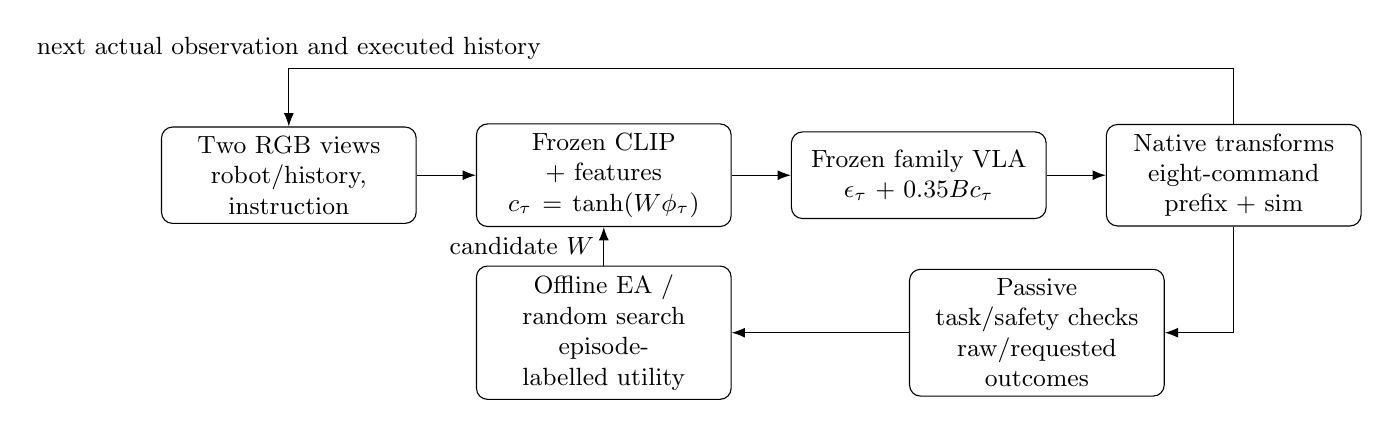
\begin{tikzpicture}[>=Latex,font=\small,
 box/.style={draw,rounded corners,align=center,minimum height=11mm,text width=30mm}]
 \node[box] (obs) at (0,0) {Two RGB views\\robot/history, instruction};
 \node[box] (adapt) at (4,0) {Frozen CLIP + features\\$c_\tau=\tanh(W\phi_\tau)$};
 \node[box] (policy) at (8,0) {Frozen family VLA\\$\epsilon_\tau+0.35Bc_\tau$};
 \node[box] (sim) at (12,0) {Native transforms\\eight-command prefix + sim};
 \node[box] (search) at (4,-2) {Offline EA / random search\\episode-labelled utility};
 \node[box] (monitor) at (9.5,-2) {Passive task/safety checks\\raw/requested outcomes};
 \draw[->] (obs) -- (adapt);
 \draw[->] (adapt) -- (policy);
 \draw[->] (policy) -- (sim);
 \draw[->] (sim.south) |- (monitor.east);
 \draw[->] (monitor) -- (search);
 \draw[->] (search) -- node[left]{candidate $W$} (adapt);
 \draw[->] (sim.north) -- ++(0,.7) -| node[pos=.5,above]{next actual observation and executed history} (obs.north);
\end{tikzpicture}
\caption{Implemented information boundary. Candidate weights are fixed within an
episode; the native Gaussian draw remains present. Outcome labels guide selection
of later candidates without vetoing execution. All conditions pay the same feature
extraction cost. The VLA also receives its unchanged native observation inputs.
No learned safety filter or world model is deployed.}
\Description{Observations feed a conditional noise controller and a frozen VLA.
Native execution feeds simulation. A passive monitor sends episode labels to the
offline search loop, which selects the next candidate controller.}
\label{fig:architecture}
\end{figure*}

\section{Native-noise controller}
\subsection{Causal features}
The feature vector $\phi_\tau\in[-1,1]^{44}$ comprises a bias, seven arm positions
divided by $\pi$, two measured finger positions divided by .04 m, seven previous
executed arm targets minus current arm positions divided by .2 rad, and three
end-effector displacements since the previous query divided by .05 m. Robot/history
coordinates are clipped. Initially the previous target equals measured joints and
displacement is zero.

The remaining 24 coordinates are eight each from overview RGB, wrist RGB and the
actual instruction. Frozen CLIP ViT-B/32~\cite{clip} produces 512-dimensional
embeddings. Each embedding is normalized to unit Euclidean norm. Fixed Gaussian-QR
projections, seeded 20261017, produce eight coordinates, multiplied by $\sqrt{512}$,
clipped to $[-5,5]$ and divided by five.
No feature fitting uses study outcomes. Images are encoded at every native query
and text once per episode, including in the native reference. The conditioning
path is implemented; its physical value is unestablished.

\subsection{Bounded steering with native stochasticity}
For genome $W\in[-1,1]^{4\times44}$, define $c_\tau=\tanh(W\phi_\tau)$ and
\begin{equation}
 z_{\tau,h}=\epsilon_{\tau,h}+.35Bc_\tau,
 \qquad h=1,\ldots,16.
 \label{eq:steering}
\end{equation}
The first seven rows of $B\in\mathbb R^{32\times4}$ are a reduced QR basis of
a Gaussian $7\times4$ matrix with PCG64 seed 20261019. Remaining rows are zero.
The offset repeats across the chunk and has Euclidean norm at most
$.35\sqrt4=.70$ per position in noise coordinates. This bounds sampling input,
not joint motion or violation probability. Gripper/padding noise are not directly
steered, but decoder coupling can affect their outputs. No persistence, learned
noise scale or activation gate is used.

For $W=0$, an explicit branch calls unchanged native \texttt{Policy.infer} without
an explicit-noise argument. Nonzero controllers preserve the native RNG split and
Gaussian draw before adding the offset. A zero noise tensor would define a different
policy. Receipts retain RNG transitions, noise/observation hashes, offsets, decoded
physical chunks and source hashes. The runtime logs steered proposals and final
environment inputs. It does not buy an additional unsteered chunk at every query;
same-noise comparisons are confined to the bounded decoder audit.

\subsection{Matched search}
Shared initialization evaluates identity, positive and negative constants, and a
uniform random conditional matrix on two cases. Constants set only
$W_{0,0}=\pm\operatorname{atanh}(.5)$, yielding $\pm.175$ along the first basis
direction. The random matrix uses seed 20261019. Both methods receive these same
eight episodes, counted once globally and attributed to both information budgets.
The better constant becomes the fixed reference, with ties selecting positive.
This tunes two declared constants, not an extensive fixed-policy baseline.

Each method evaluates two generations of four candidates on two common cases per
generation. Both freshly re-evaluate the previous cohort's best candidate. EA adds
three children from alternating top-two parents using iid Gaussian weight mutation
with standard deviation .25 and clipping to $[-1,1]$. Random search instead draws
three uniform matrices from the same domain, with the same retained-incumbent cost.
Ranking uses summed utility and stable identifiers for ties. Only the last complete
cohort supplies each finalist, preventing best-of-repeat promotion. Both method
RNGs use seed 20261020. Descendant execution interleaves methods at each candidate
slot, using EA/random at even slots and random/EA at odd slots. Lineage and
pending/completed evaluations are persisted.

\begin{algorithm}[t]
\caption{Frozen comparison after four development episodes}
\label{alg:comparison}
\begin{algorithmic}[1]
\Require Pinned policy, features, domain, cases, seeds and budget
\State Evaluate four shared controllers on two cases (8 episodes)
\State Select fixed reference from the two constants
\State Initialize EA and random search with the same scored data
\For{generation $g=1,2$}
 \State Propose both four-candidate cohorts, including incumbents
 \For{candidate slot $j=0,1,2,3$}
  \For{method in the frozen alternating slot order}
   \State Evaluate its candidate on two common cases
   \State Verify both physical receipts and record scores
  \EndFor
 \EndFor
 \State Rank each complete cohort for subsequent selection
 \State Preserve all attempts, ancestry, RNG and physical records
\EndFor
\State Seal native, fixed and the two final-cohort finalists
\State Check four conditions on four blocks (16 episodes)
\State Report outcomes, block differences, activity and costs
\end{algorithmic}
\end{algorithm}

\section{Prospectively frozen physical protocol}
\subsection{Scope and native execution}
Jar and Clutter provide development exposure; Cabinet and Dusty remain physically
untouched by this study. Jar/Stack/Lid/Clutter have programme-level history.
Jar is the primary pilot and Clutter the declared capacity fallback. The selected
protocol was frozen at 04:27:23 UTC on 20 October before comparative feedback,
using development timing and the authority criterion. It selects Jar. This pilot
does not train or test one shared cross-family adapter.

Execution uses native $640\times640$ DLAA rendering, two actual camera views,
the verified extended-finger Franka, assisted grasping, 20 Hz policy control,
60 Hz rendering and 120 Hz physics. Hard horizons are 2,000 controls for Jar and
1,100 for Clutter. Preprocessing, gripper binarization, native clipping and
termination are unchanged. Jar uses checkpoint step 7400, revision
\texttt{1d84eda07031}; Clutter uses step 7100, \texttt{f572e33bdb49}.
Full revisions and file hashes remain in study records.

Jar training tasks are 0019/0009, with base seeds $6101910+10g+i$, generation
$g=0,1,2$ and task index $i=0,1$. Checking tasks 0016/0012/0011/0003 use seeds
$6101940+i$. These blocks are reserved from this optimizer's feedback. Historical
validation allocation does not establish absence of earlier programme exposure;
we conservatively describe them as exposed tasks with independent checking.
The original main-study test partition remains excluded. Native per-scene
sampling-seed derivation is retained.

\subsection{Allocation and hardware balancing}
Table~\ref{tab:allocation} specifies the 60 planned valid full episodes. At most
four genuine infrastructure failures may be replaced, yielding a 64-full-attempt
ceiling. Every partial/invalid attempt and discarded candidate is charged. Valid
timeouts and adverse scores cannot be replaced. Separate engineering used six
starts: three failed during preparation and three reached 32 controls each.
The 96-control engineering allowance is exhausted. Physics before callback
attachment is unknown, not zero. No further decoder probes are allowed.

\begin{table}[t]
\caption{Frozen full-episode allocation. Shared initialization is acquired once.
The sixteen-episode independent check is protected from adaptation and tuning.}
\label{tab:allocation}
\begin{tabular}{@{}p{\dimexpr\columnwidth-65pt\relax}r@{}}
\toprule
Stage & Valid episodes \\
\midrule
Development, Jar + Clutter & 4 \\
Shared initialization: four controllers, two cases & 8 \\
EA: two generations, four candidates, two cases & 16 \\
Random search: same structure and domain & 16 \\
Independent check: four conditions, four blocks & 16 \\
\midrule
Planned total & 60 \\
Maximum starts with infrastructure replacements & 64 \\
\bottomrule
\end{tabular}
\end{table}

Two workers each colocate simulation and policy on one RTX 3090. Training case
$i$ uses worker $(i+g)\bmod2$ for both methods. Denoting native, fixed, EA and
random by $N,F,E,R$, checking orders are $(N,F,E,R)$, $(F,R,N,E)$,
$(E,N,R,F)$ and $(R,E,F,N)$. Adjacent pairs run concurrently; positions zero and two
use worker zero. Every condition therefore runs twice per GPU. One admission
ledger enforces the global attempt ceiling. Process identities and terminal
receipts permit reattachment without duplicate physical launches.

Capacity protects 56 post-development episodes plus four replacement slots as 30
two-worker waves. Its per-wave bound is the maximum of 180 s, 1.25 times the
slowest complete development process, and a startup-plus-native-horizon throughput
estimate with the same margin. Including 900 s for lifecycle/preservation, Jar
requires 15.008 h. The original window was insufficient; the user subsequently
authorized the full comparison on this instance. The fixed cutoff is 19:30 UTC
and independent local stop 20:00 UTC on 20 October. Horizons/rendering were not
reduced to fit.

\subsection{Analysis and uncertainty}
The final comparison will retain all four requested completion and safety categories
and raw benchmark completion per condition, with paired differences by checking
block. Initial robot/image hashes are checked: common seeds do not prove identical
camera observations. Contact/grasp indicators contextualize noncompletion.
Cost curves use common cumulative physical control counts and retain all adaptation,
failures and discarded candidates. Model calls, encoder work, elapsed time and
allocated GPU-hours are separate counters. Shared episodes count once physically
and once within each method's information budget.

Setup, decoder calls, idle allocation and preservation are charged. Rental-wall
estimates retain the original provider start; any stopped interval needs separate
billing reconciliation rather than resetting the clock. Four checking episodes
per condition and one optimizer seed provide descriptive effect sizes, not a
superiority or safety guarantee. Zero violations in $n$ independent episodes
implies an approximate 95\% upper rate bound of $3/n$, not zero; four episodes
are particularly weak evidence.

\section{Completed development evidence}
\subsection{Identity and decoder influence}
Eight saved observations per family, from two development tasks, each use two native
noise draws. Each draw receives two same-noise baselines and positive/negative
offsets along four directions: ten calls and 320 total. All sixteen identity pairs
per family pass the declared $10^{-5}$ absolute/relative tolerance. Full remote
recovery also reproduces noise hashes and RNG transitions without new model calls.

\begin{figure}[t]
\centering
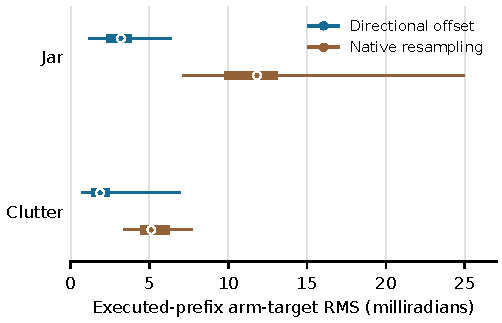
\includegraphics[width=\linewidth]{decoder-authority.pdf}
\caption{Arm-target RMS differences over the executed eight-command prefix.
Thick intervals show quartiles, thin intervals the range and circles the median.
There are 128 directional comparisons and eight native-resampling comparisons per
family, clustered within eight saved observations. These are decoder responses,
not independent physical trials or safety measurements.}
\Description{Jar perturbation median is .00319 rad versus .01183 for native
resampling; Clutter medians are .00187 and .00512 rad, respectively.}
\label{fig:authority}
\end{figure}

Perturbed-prefix arm RMS ranges from .001131 to .006422 rad for Jar, median
.003193, and .000666 to .006975 rad for Clutter, median .001868
(Figure~\ref{fig:authority}). Native-resampling medians are .011827/.005118 rad.
All four directions per family pass the frozen criterion: observation-level mean
RMS at least .001 rad on at least half the observations, with two passing
directions required. The smallest individual Clutter response need not exceed
this observation-level threshold. No executed-prefix gripper flips occur among
128 directional probes per family. Coupling elsewhere is not excluded.

A 32-control Clutter integration check uses an untrained dense conditional matrix,
exercising all 176 weights including 96 semantic weights. Removing semantic
features offline changes its code by RMS .3781 on factual observations. This
verifies a software path, not semantic competence or a physical counterfactual.

\subsection{Full development outcomes}
Table~\ref{tab:development} preserves four full episodes on different tasks/seeds.
Their native/bias differences do not estimate an adaptation effect. Jar native
reaches the raw benchmark goal but fails the closed-lid sequence: requested unsafe
unfinished, versus raw unsafe completion. Jar bias and Clutter native reach their
full horizons, both valid outcomes rather than replaceable failures.

\begin{table}[t]
\caption{Full development episodes. $C$ is requested completion, $V$ raw
violation, $A$ controls and $Q$ policy calls. Each row uses a different task/seed.}
\label{tab:development}
\begin{tabular}{llrrrrr}
\toprule
Family/controller & Task & $A$ & $Q$ & $C$ & $V$ & $U$ \\
\midrule
Jar native & 0013 & 666 & 84 & 0 & 1 & $-2$ \\
Jar positive bias & 0017 & 2000 & 250 & 0 & 0 & 0 \\
Clutter native & 0039 & 1100 & 138 & 0 & 1 & $-2$ \\
Clutter negative bias & 0010 & 532 & 67 & 1 & 0 & 1 \\
\bottomrule
\end{tabular}
\end{table}

Development closeout contains ten starts, 4,394 controls, 4,464 environment steps
and 26,987 known physics ticks. There are 551 physical-policy calls and 320 decoder
calls. Encoding records 1,102 images, seven text calls, 23.519 s extraction and
38.443 s loading; physical-policy request wall time is 293.776 s. These totals
precede the running comparison and are not final study costs. Callback-unobserved
initialization physics remains unknown.

Clutter native has a 574.6 s cold startup versus its partner's 99.9 s. Logs identify
a locked shared Kit cache and shader compilation. The episode then completes
normally and retains its cost in capacity selection. This technical delay is
distinct from its valid adverse physical outcome.

\subsection{Comparison in progress}
\textbf{Optimizer and independent comparison results are pending.} Jar shared
initialization began at 04:28 UTC on 20 October with two concurrent native episodes.
At this draft's evidence cutoff no EA/random-search finalist is selected. We leave
comparative rates, optimizer differences and transfer results unreported. Training
observations will not substitute for the protected sixteen-episode final check.

\section{Limitations and remaining evidence}
This interface can consume several family checkpoints, but the pilot fits only
within Jar. A random four-direction basis may miss useful behaviour. A bounded
noise offset need not imply safe contact dynamics. The 176-parameter domain is
large relative to two-case candidate feedback. Noisy selection, adverse behaviour
and identity finalists are valid outcomes. If a constant explains an improvement,
conditioning is unestablished; if random search matches EA, evolutionary advantage
is unestablished.

An episodic parameter-REINFORCE interface over the same bounded matrix is implemented
and CPU-checked, including interrupted-batch recovery. It has zero physical
evaluations and is outside the frozen minimum allocation. It does not replace a
competent state-conditioned DSRL-style latent SAC baseline. That baseline, matched
tuning and independent optimizer replication are required before claiming practical
evolutionary superiority. A direct-action residual baseline is additionally needed
to attribute any advantage to the latent representation.

The cross-family target requires freezing one fitted controller and checking new
tasks and an adaptation-held-out family with its own frozen base policy.
Response-informed bases, persistence, sampling-distribution control and internal
activation gates remain prospective, with no physical result here. A proposed
156-episode adaptation/transfer bridge is separately budgeted and unexecuted.
Neither extensions nor tuning may consume the final checking allowance.

\section{Reproducibility and preservation}
The launch revision is \texttt{4783369c5b59}. Upstream pins are ManiGuard
\texttt{6bf4c61a1f16}, BEHAVIOR \texttt{88454bd04f75} and openpi
\texttt{215abfb217db}~\cite{openpi}. Separate uv-managed environments serve
simulation (Python 3.10, Torch 2.6/CUDA 12.4), policy (Python 3.11, JAX .5.3) and
CPU tooling. Receipts retain actual GPU UUIDs, source hashes, causal features,
decoded chunks, executed inputs and raw/requested outcome evidence. An independent
reader verifies physical records before assigning fitness.

Code, compact evidence and frozen protocols are preserved in
\url{https://github.com/Sachin2911/Safety-Dial}. The protocol is
\path{configs/maniguard/latent-evolution/capacity-20261020-v2.json}; its study README
documents reconstruction. Separate private Hugging Face model/dataset repositories
store immutable stage archives with remote revision, privacy, size and SHA-256
verification. Full recovery reconstructs development records and all 32 identity
pairs without new physics or model calls. Raw runs, licensed assets, credentials
and base-policy weights are excluded from public Git.

\section{Conclusion}
Native-noise steering is implemented with conditional inputs and verified decoder
influence in two family policies. These checks justify a physical test without
establishing safer completion. The frozen Jar comparison tests native execution,
a tuned constant, evolution and matched random search while protecting independent
checking and retaining unsuccessful candidates. Its result must determine the
strength of the contribution, including a null or adverse finding. Ordinary
learning, replication and transfer remain necessary for the broader claim.

\begin{acks}
This BSc Honours research at the University of the Witwatersrand is supervised by
Geraud Nangue Tasse. AI coding assistance supported implementation, diagnosis and
drafting; recorded empirical evidence and its stated limits govern the claims.
\end{acks}
\bibliographystyle{ACM-Reference-Format}
\bibliography{references,latent-references}
\end{document}
